
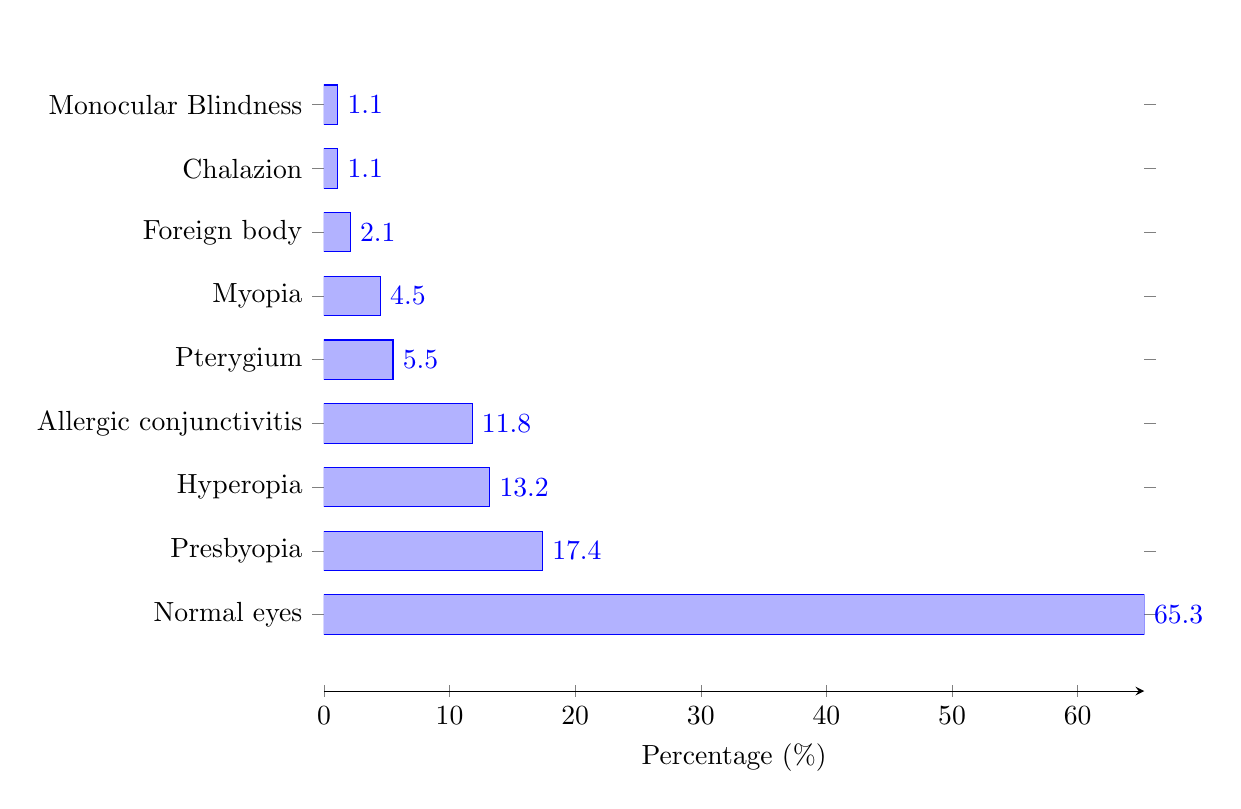
\begin{tikzpicture}
\begin{axis}[
    xbar,
    width=12cm, % Adjust the width to fit your needs
    height=10cm, % Adjust the height to fit your needs
    xlabel={Percentage (\%)},
    symbolic y coords={Normal eyes, Presbyopia, Hyperopia, Allergic conjunctivitis, Pterygium, Myopia, Foreign body, Chalazion, Monocular Blindness},
    ytick=data,
    nodes near coords,
    nodes near coords align={horizontal},
    xmin=0, % Start x-axis from 0
    bar width=0.5cm, % Adjust the bar thickness
    y axis line style={opacity=0},
    axis x line=bottom,
    enlarge y limits=0.15,
]

\addplot coordinates {(65.3,Normal eyes) (17.4,Presbyopia) (13.2,Hyperopia) (11.8,Allergic conjunctivitis) (5.5,Pterygium) (4.5,Myopia) (2.1,Foreign body) (1.1,Chalazion) (1.1,Monocular Blindness)};

\end{axis}
\end{tikzpicture}

